\def\fpn{
    Các kiến trúc mô hình xương sống\index{mô hình xương sống} như AlexNet\index{AlexNet} \cite{krizhevsky2012imagenet}, VGG\index{VGG} \cite{simonyan2014very}, InceptionNet\index{InceptionNet} \cite{szegedy2015going}, SqueezeNet\index{SqueezeNet} \cite{iandola2016squeezenet} và đặc biệt là ResNet\index{ResNet} \cite{he2016deep} đã đạt những thành công nhất định.
    Tuy nhiên, các kiến trúc mô hình xương sống\index{mô hình xương sống} trên vẫn gặp phải một vấn đề về chênh lệch kích thước giữa các đối tượng trong ảnh.
    Feature Pyramid Networks\index{Feature Pyramid Networks} \cite{lin2017feature} (gọi tắt là FPN\index{FPN}) được giới thiệu như một kiến trúc mô hình xương sống\index{mô hình xương sống} nhằm giải quyết vấn đề trên.
    Việc sử dụng FPN\index{FPN} như là kiến trúc mô hình xương sống\index{mô hình xương sống} kết hợp cùng mô hình Faster R-CNN\index{Faster R-CNN}\index{Faster R-CNN} \cite{ren2015faster} đã vượt qua rất nhiều các mô hình nhận diện đối tượng\index{nhận diện đối tượng} khác để trở thành mô hình tốt nhất ở thời điểm đó.

    \subsubsection*{So sánh các kiến trúc pyramid\index{kiến trúc pyramid} khác nhau}

    \begin{figure}[H]
        \centering
        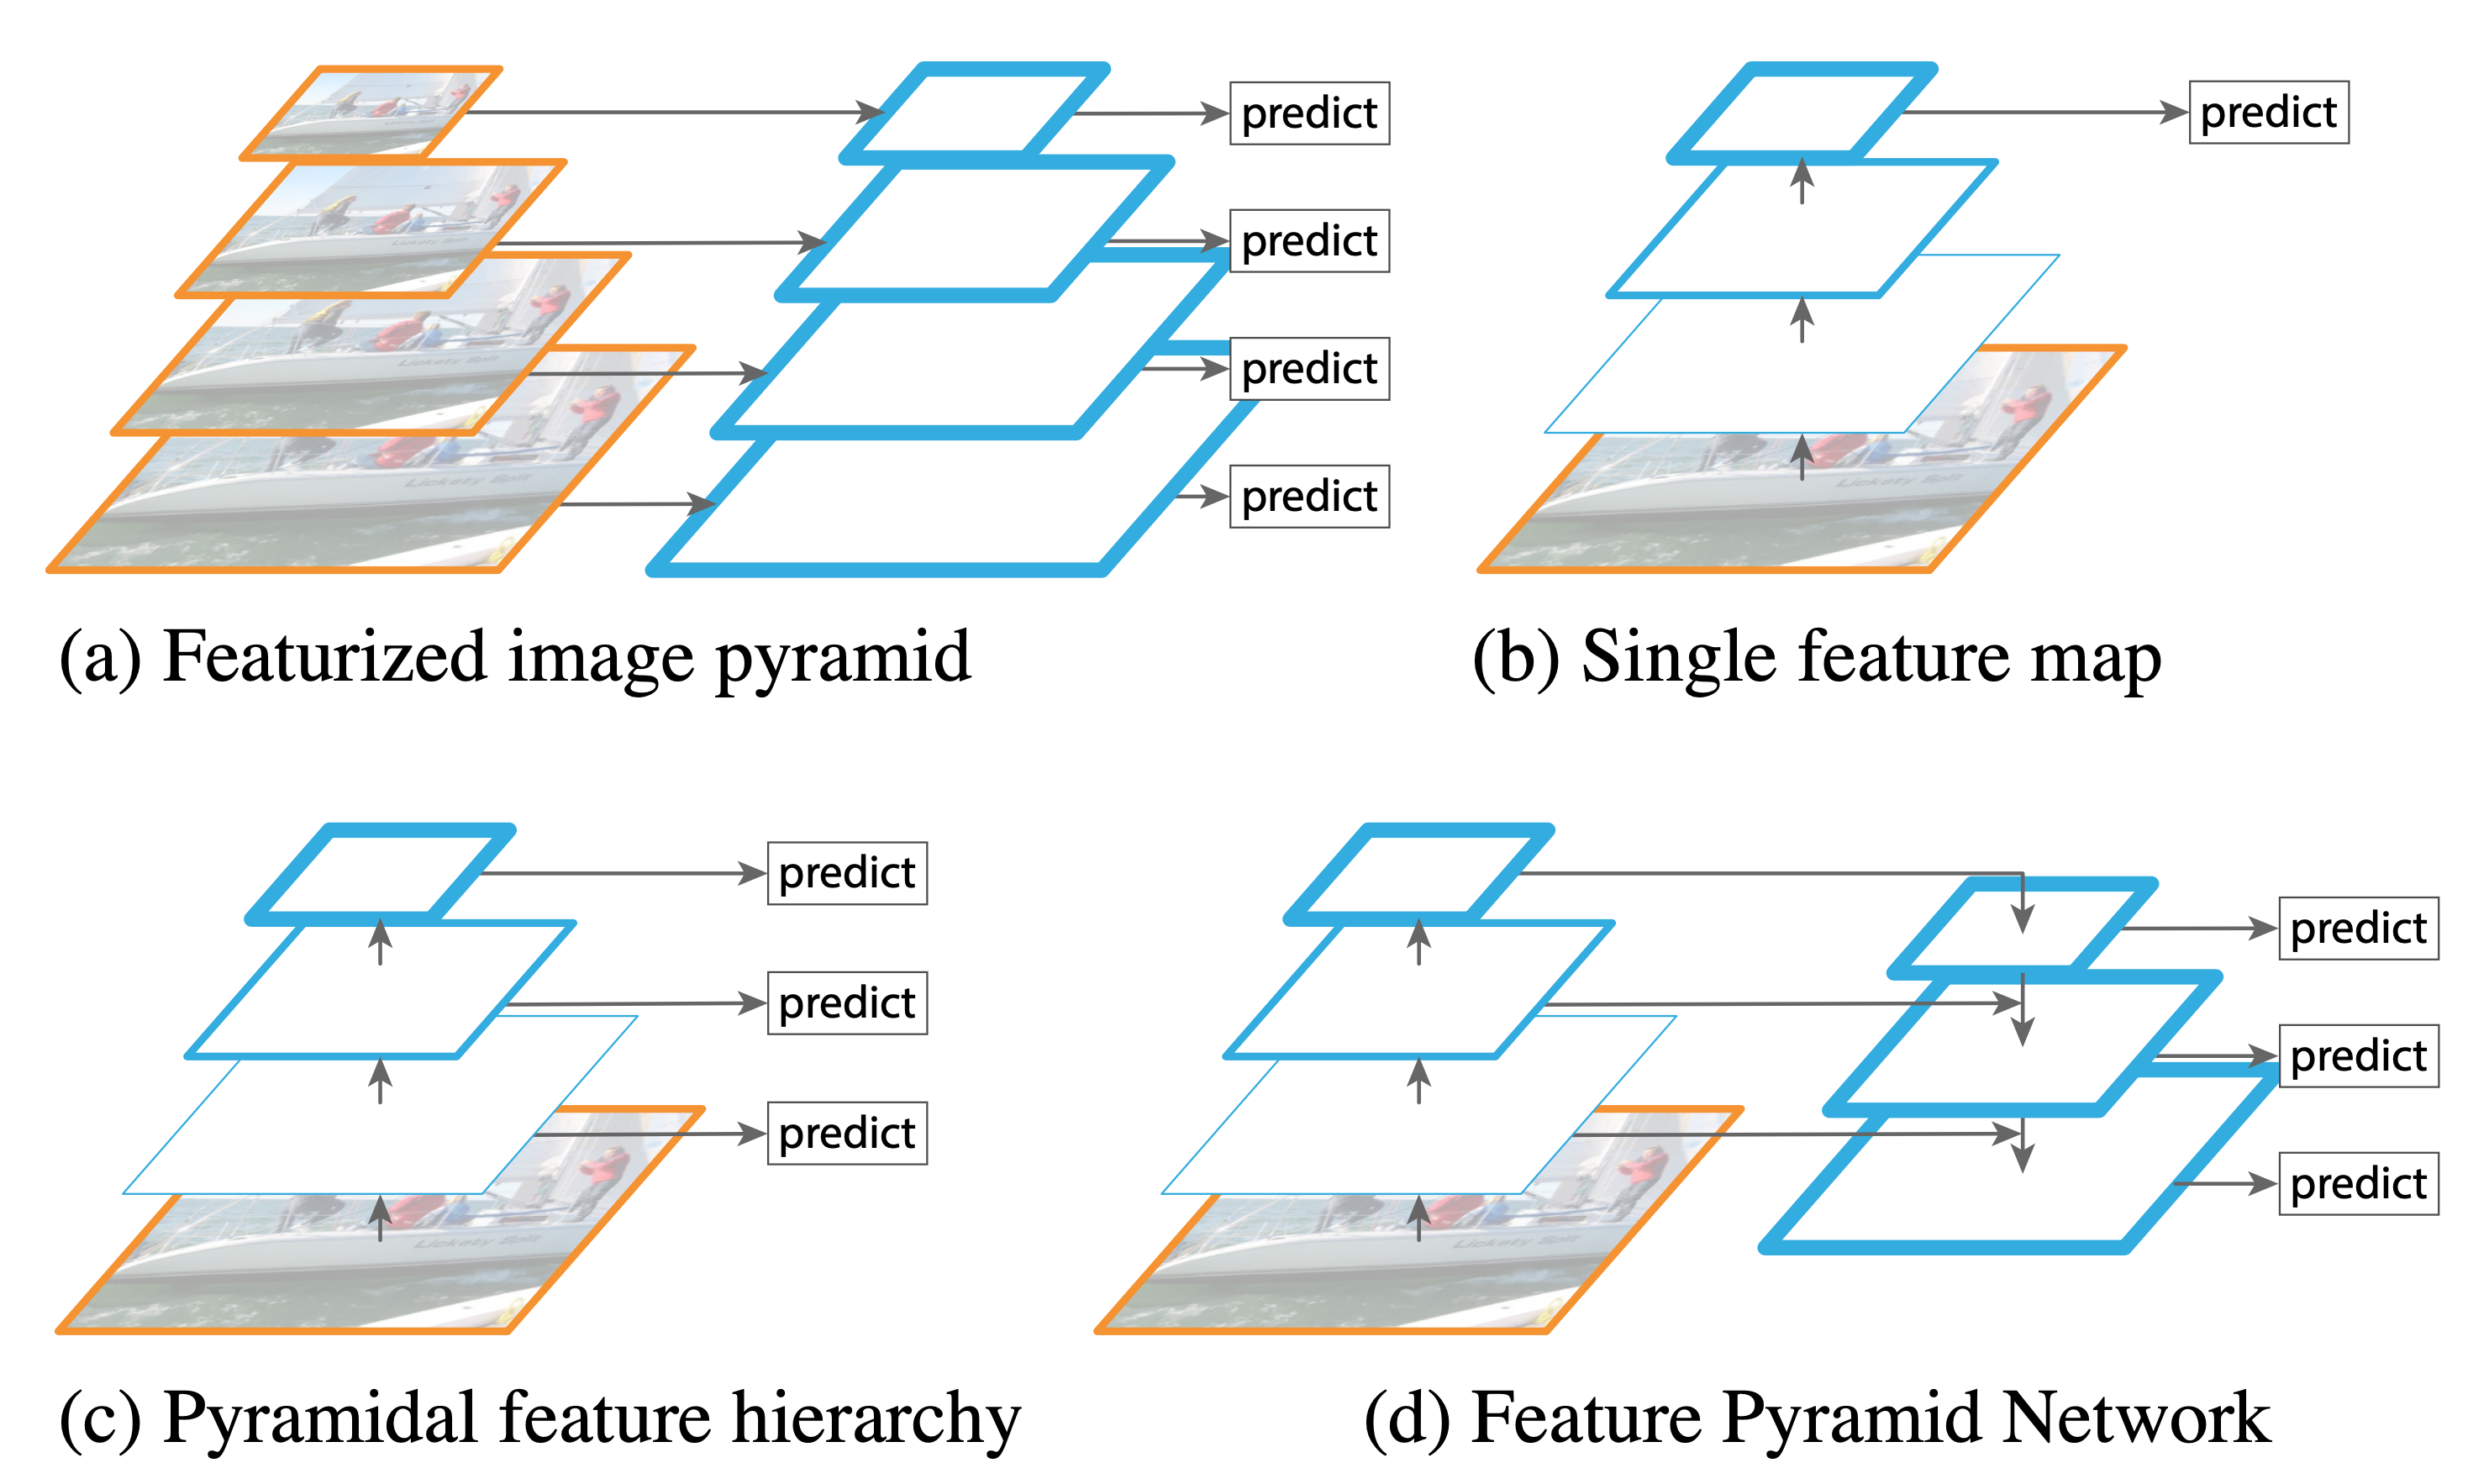
\includegraphics[width=12cm] {images/fpn_compare}
        \caption{So sánh các kiến trúc pyramid\index{kiến trúc pyramid} khác nhau (Nguồn: \cite{lin2017feature})}
        \label{fig:fpn_compare}
    \end{figure}

    \noindent
    Ý tưởng về việc xây dựng và sử dụng các đặc trưng của ảnh với nhiều kích thước khác nhau không mới, tuy nhiên, các giải pháp đã có vào thời điểm đó đều vướng phải một số vấn đề: \\
    - \textit{Featurized image pyramid}\index{Featurized image pyramid}: Việc sử dụng nhiều kích thước ảnh khác nhau để tạo ra nhiều đặc trưng có kích thước khác nhau một cách độc lập là ý tưởng cơ bản nhất. Mặc dù đạt được hiệu quả cao về độ chính xác khi khai thác ảnh đầu vào với nhiều kích thước khác nhau, nhưng phương pháp này khiến cho mô hình giải bài toán nhận diện đối tượng\index{nhận diện đối tượng} trở nên cồng kềnh và tốn rất nhiều thời gian để xử lý và gần như bất khả thi để có thể huấn luyện được mô hình. \\
    - \textit{Single feature map}\index{Single feature map}: Việc sử dụng chỉ một kích thước đặc trưng duy nhất giúp cho mô hình xử lý nhanh hơn nhưng lại khiến cho mô hình khó có thể học được những đặc trưng giữa các đối tượng có kích thước chênh lệch trong ảnh. Đặc biệt, việc đưa ảnh đầu vào qua nhiều khối Conv đã loại bỏ rất nhiều thông tin và gần như không còn thông tin để mô hình có thể nhận biết được các đối tượng có kích thước nhỏ. \\
    - \textit{Pyramidal feature hierarchy}\index{Pyramidal feature hierarchy}: Việc sử dụng nhiều bản đồ đặc trưng\index{bản đồ đặc trưng} có kích thước khác nhau cùng đưa ra kết quả được sử dụng trong mô hình nhận diện đối tượng\index{nhận diện đối tượng} khá nổi tiếng là SSD \cite{liu2016ssd}. Tuy nhiên, thay vì tận dụng toàn bộ các bản đồ đặc trưng\index{bản đồ đặc trưng} sinh ra từ các khối Conv của mô hình xương sống\index{mô hình xương sống} VGG-16\index{VGG-16}, SSD chỉ sử dụng bản đồ đặc trưng\index{bản đồ đặc trưng} từ khối Conv thứ năm và bổ sung thêm các lớp Conv\index{lớp Conv}. Điều này khiến cho SSD bỏ qua những bản đồ đặc trưng\index{bản đồ đặc trưng} có kích thước lớn, có ý nghĩa quan trọng trong việc detect các đối tượng có kích thước nhỏ. \\
    - \textit{Feature Pyramid Network}\index{Feature Pyramid Network}: Dựa trên vấn đề trên từ SSD, nhóm tác giả đề xuất FPN\index{FPN} tận dụng tối đa các bản đồ đặc trưng\index{bản đồ đặc trưng} trích xuất được từ mô hình xương sống\index{mô hình xương sống} nhằm tạo ra bộ bản đồ đặc trưng\index{bản đồ đặc trưng} mới gồm nhiều kích thước khác nhau và chứa rất nhiều thông tin về nội dung của ảnh đầu vào. Để đạt được điều này, nhóm tác giả thiết kế kiến trúc kết hợp những bản đồ đặc trưng\index{bản đồ đặc trưng} có kích thước lớn và những bản đồ đặc trưng\index{bản đồ đặc trưng} có kích thước nhỏ bằng đường mô hình trên xuống\index{đường mô hình trên xuống} và đường kết nối lateral\index{đường kết nối lateral}.

    \subsubsection*{Chi tiết kiến trúc FPN}
    Ý tưởng về việc sử dụng kiến trúc mô hình theo dạng từ trên xuống không phải là mới và đã được nhắc đến trong một số nghiên cứu. Tuy nhiên, điểm giống nhau của các nghiên cứu có thiết kế mô hình theo kiểu từ trên xuống đó là mô hình chỉ sử dụng một bản đồ đặc trưng\index{bản đồ đặc trưng} cuối cùng, sau khi đã tổng hợp các thông tin trong suốt quá trình từ trên xuống, để đưa ra quyết định dự đoán cuối cùng.

    \noindent
    Trong khi đó, đối với FPN, nhóm tác giả đưa ra quyết định dự đoán trên từng bản đồ đặc trưng\index{bản đồ đặc trưng} trong suốt quá trình từ trên xuống. Từ đó, đặc biệt nâng cao chất lượng của mô hình nhận diện đối tượng\index{nhận diện đối tượng} khi có thể vừa trích xuất được thông tin của các đối tượng có kích thước lớn từ các bản đồ đặc trưng\index{bản đồ đặc trưng} có kích thước nhỏ vừa trích xuất được thông tin của các đối tượng có kích thước nhỏ từ các bản đồ đặc trưng\index{bản đồ đặc trưng} có kích thước lớn.

    \begin{figure}[H]
        \centering
        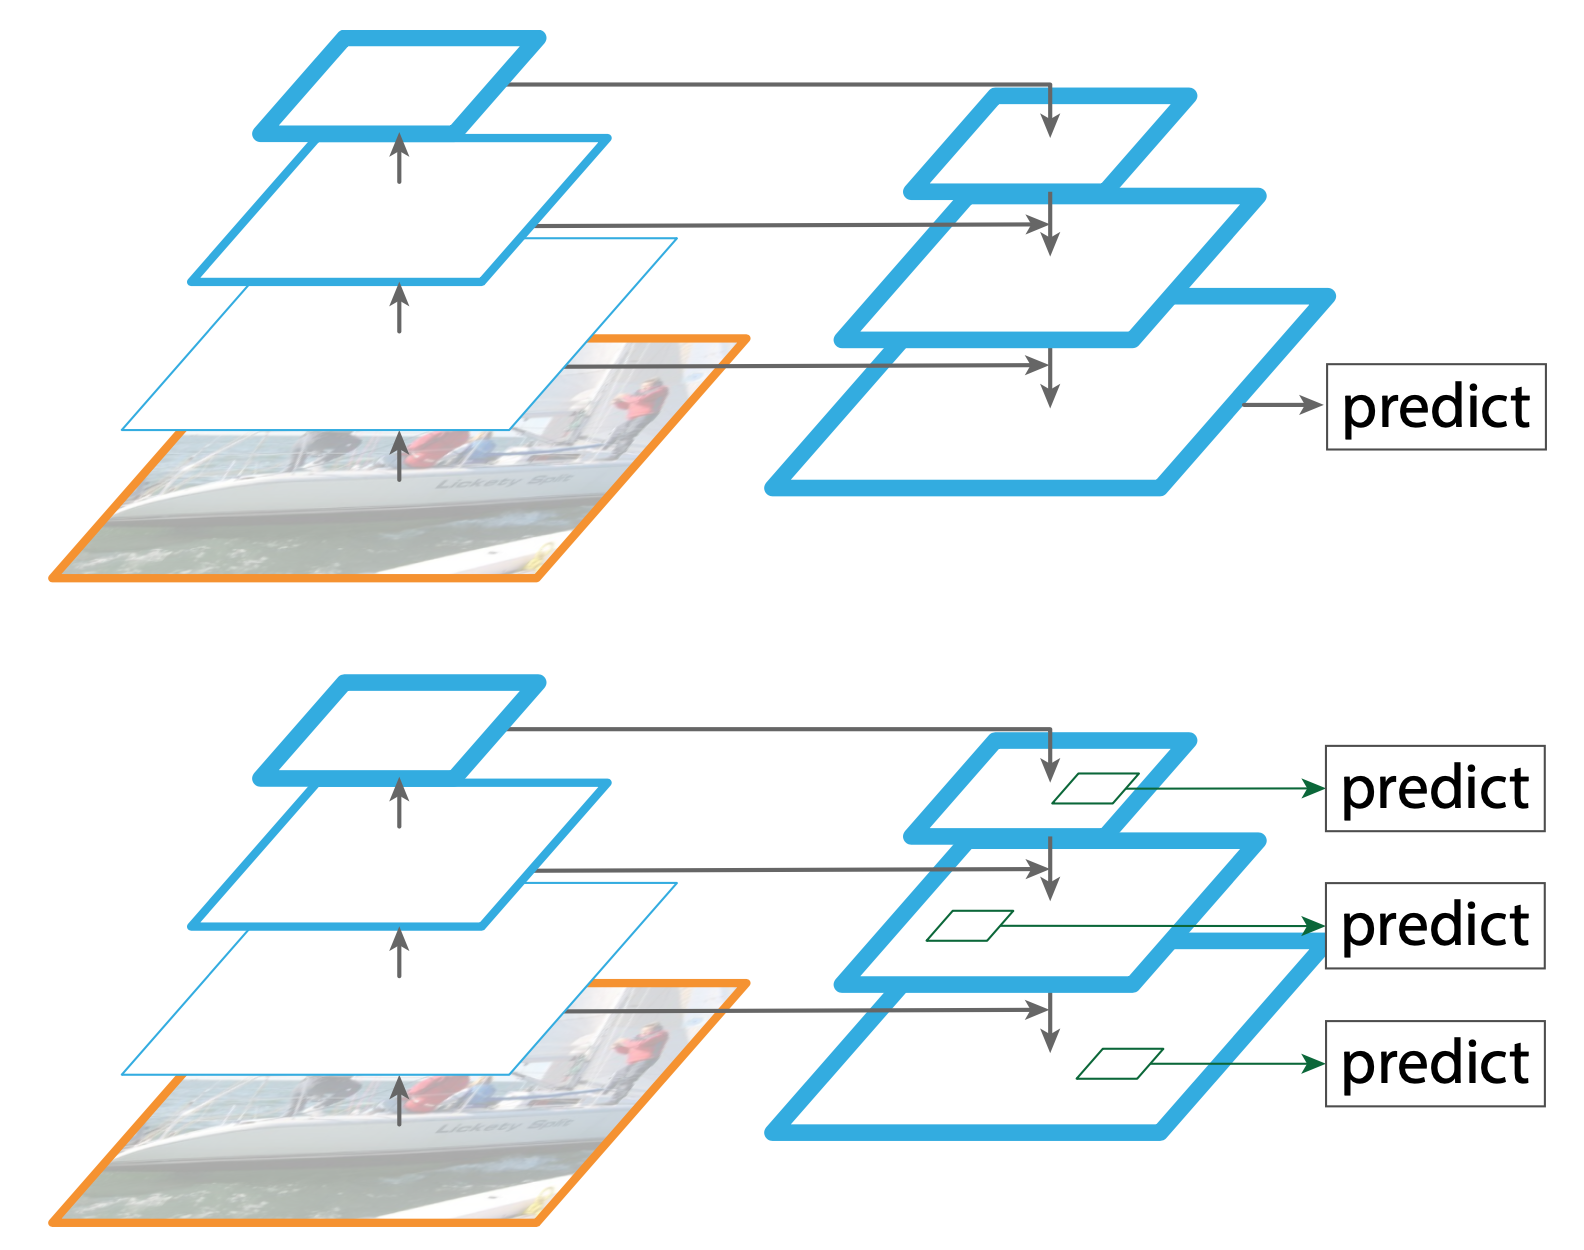
\includegraphics[width=8cm] {images/fpn_topdown}
        \caption{So sánh các kiến trúc theo dạng từ trên xuống khác nhau (Nguồn: \cite{lin2017feature})}
        \label{fig:fpn_topdown}
    \end{figure}

    \noindent
    Kiến trúc FPN\index{FPN} có thể được áp dụng với nhiều mô hình xương sống\index{mô hình xương sống} Conv khác nhau như AlexNet, VGG hay ResNet, cụ thể trong nghiên cứu, nhóm tác giả lựa chọn ResNet làm mô hình mô hình xương sống.
    Kiến trúc FPN\index{FPN} có thể được chia làm hai phần: \\
    - \textit{Đường mô hình dưới lên}\index{đường mô hình dưới lên} là quá trình mà ta đưa ảnh đầu vào qua mô hình mô hình xương sống\index{mô hình xương sống} Conv như ResNet và thu được các bản đồ đặc trưng\index{bản đồ đặc trưng}.
    Tuy nhiên, trong các mô hình mô hình xương sống\index{mô hình xương sống} Conv, sẽ có một nhóm các lớp Conv\index{lớp Conv} tạo ra các bản đồ đặc trưng\index{bản đồ đặc trưng} có kích thước giống nhau, và nhóm các lớp Conv\index{lớp Conv} này được gọi là một khối Conv.
    Đối với FPN, nhóm tác giả lựa chọn các bản đồ đặc trưng\index{bản đồ đặc trưng} được sinh ra từ các lớp Conv\index{lớp Conv} cuối cùng trong mỗi khối Conv để sử dụng cho nhánh đường mô hình trên xuống\index{đường mô hình trên xuống}.
    Cụ thể đối với mô hình mô hình xương sống\index{mô hình xương sống} ResNet, nhóm tác giả sử dụng các bản đồ đặc trưng\index{bản đồ đặc trưng} được sinh ra từ residual block cuối cùng của mỗi khối Conv (trừ khối Conv đầu tiên do kích thước của bản đồ đặc trưng\index{bản đồ đặc trưng} này lớn và gây ra vấn đề về bộ nhớ), ký hiệu là \textit{{${C}_{2}, {C}_{3}, {C}_{4}, {C}_{5}$}}.
    Các bản đồ đặc trưng\index{bản đồ đặc trưng} này có kích thước lần lượt bằng 1/4, 1/8, 1/16 và 1/32 so với kích thước của ảnh đầu vào.

    \begin{figure}[H]
        \centering
        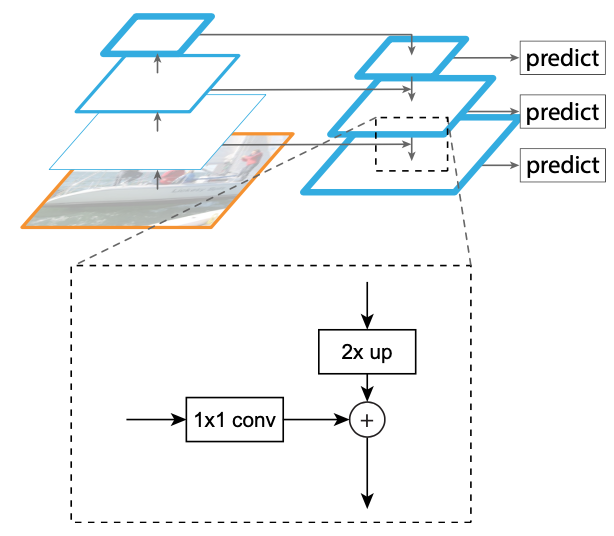
\includegraphics[width=8cm] {images/fpn_detail}
        \caption{Chi tiết kiến trúc FPN (Nguồn: \cite{lin2017feature})}
        \label{fig:fpn_detail}
    \end{figure}

    \noindent
    - \textit{Đường mô hình trên xuống và đường kết nối lateral}\index{đường mô hình trên xuống}\index{đường kết nối lateral} là quá trình mà FPN\index{FPN} sinh ra thêm các bản đồ đặc trưng\index{bản đồ đặc trưng} mới từ các bản đồ đặc trưng\index{bản đồ đặc trưng} của đường mô hình dưới lên\index{đường mô hình dưới lên} và kết hợp chúng lại thông qua đường kết nối lateral\index{đường kết nối lateral}.
    Cụ thể, các bản đồ đặc trưng\index{bản đồ đặc trưng} của đường mô hình dưới lên\index{đường mô hình dưới lên} được đưa qua các lớp Conv\index{lớp Conv} có kích thước 1x1, stride\index{stride} bằng một nhằm giữ nguyên kích thước chiều dài, chiều rộng và chỉ thay đổi kích thước chiều channel\index{channel} của bản đồ đặc trưng\index{bản đồ đặc trưng}.
    Các bản đồ đặc trưng\index{bản đồ đặc trưng} ở vị trí cao hơn (có kích thước nhỏ hơn) được upsample\index{upsample} thông qua thuật toán người hàng xóm gần nhất\index{thuật toán người hàng xóm gần nhất} và cộng ma trận với bản đồ đặc trưng\index{bản đồ đặc trưng} đầu ra từ lớp Conv\index{lớp Conv} 1x1 nói trên.
    Cuối cùng, các bản đồ đặc trưng\index{bản đồ đặc trưng} đầu ra từ phép cộng ma trận nói trên được đi qua một lớp Conv\index{lớp Conv} 3x3 có cùng số đầu ra channel\index{channel} của bản đồ đặc trưng\index{bản đồ đặc trưng} nhằm giảm bớt hiệu ứng của thuật toán người hàng xóm gần nhất\index{thuật toán người hàng xóm gần nhất} và tạo ra các bản đồ đặc trưng\index{bản đồ đặc trưng} đầu ra cuối cùng có cùng số channel\index{channel} với nhau.
    Tập hợp bản đồ đặc trưng\index{bản đồ đặc trưng} này được gọi là \textit{{${P}_{2}, {P}_{3}, {P}_{4}, {P}_{5}$}} tương ứng với các bản đồ đặc trưng\index{bản đồ đặc trưng} có cùng kích thước \textit{{${C}_{2}, {C}_{3}, {C}_{4}, {C}_{5}$}}.

    \subsubsection*{Vấn đề tồn đọng của kiến trúc FPN}
    Kiến trúc FPN ra đời đã tạo ra một trong số những kiến trúc mô hình xương sống\index{mô hình xương sống} kinh điển trong bài toán nhận diện đối tượng\index{nhận diện đối tượng} nói riêng.
    Kiến trúc FPN đã giúp cho nhiều mô hình đạt độ chính xác cao hơn và trong khi tốc độ của mô hình không bị tăng một cách đáng kể.
    Tuy nhiên, đối với cụ thể bài toán nhận diện đối tượng\index{nhận diện đối tượng}, việc kết hợp kiến trúc FPN vào mô hình Faster R-CNN\index{Faster R-CNN} mới chỉ cải thiện về mặt độ chính xác cho mô hình Faster R-CNN\index{Faster R-CNN} mà chưa giúp tăng tốc mô hình Faster R-CNN\index{Faster R-CNN}.
    Vẫn còn một câu hỏi cần phải được giải quyết đó là làm sao để duy trì được độ chính xác mà FPN mang lại những mô hình nhận diện đối tượng\index{nhận diện đối tượng} vẫn có để đạt tốc độ nhanh hơn nữa.
}